% ****************************************************************************************** % Dissertation template and document class for Princeton University
% Author  : Jeffrey Scott Dwoskin <jdwoskin@princeton.edu>
% Adapted from: http://www.math.princeton.edu/graduate/tex/puthesis.html
% ****************************************************************************************** %


%%% For print copies
%% set 'singlespace' option to set entire thesis to single space, and define "\printmode" to remove all hyperlinks for printed copies of the thesis. Delete all output files before changing this mode -- it will turn hyperref package on and off
%\documentclass[12pt,lot, lof, singlespace]{puthesis}
%\newcommand{\printmode}{}

%%% For the electronic copy, use doublespacing, define "\proquestmode" to use outlined links, instead of colored links. 
\documentclass[12pt,lot, lof]{puthesis}
\newcommand{\proquestmode}{}
% I prefer proquestmode to be off for electronic copies for normal use, since the colored links are less distracting. However when printed in black and white, the colored links are difficult to read. 

%%% For early drafts without some of the frontmatter
% Also see the "ifodd" command below to disable more frontmatter
%\documentclass[12pt]{puthesis}

%%%%%%%%%%%%%%%%%%%%%%%%%%%%%%%%%%%%%%%%%%%%%%%%%%%%%%%%%%%%%\
%%%% Author & title page info

\title{Particle Filter Localization for Quadcopters Using Augemented Reality Tags}

\submitted{May 2013}  % degree conferral date (January, April, June, September, or November)
\copyrightyear{2013}  % year in which the copyright is secured by publication of the dissertation.
\author{Edward Francis Kelley V}
\adviser{Professor Szymon Rusinkiewicz}  %replace with the full name of your adviser
%\departmentprefix{Program in}  % defaults to "Department of", but programs need to change this.
\department{Computer Science}

%%%%%%%%%%%%%%%%%%%%%%%%%%%%%%%%%%%%%%%%%%%%%%%%%%%%%%%%%%%%%\
%%%% Tweak float placements
% From: http://mintaka.sdsu.edu/GF/bibliog/latex/floats.html "Controlling LaTeX Floats"
% and based on: http://www.tex.ac.uk/cgi-bin/texfaq2html?label=floats
% LaTeX defaults listed at: http://people.cs.uu.nl/piet/floats/node1.html

% Alter some LaTeX defaults for better treatment of figures:
    % See p.105 of "TeX Unbound" for suggested values.
    % See pp. 199-200 of Lamport's "LaTeX" book for details.
    %   General parameters, for ALL pages:
    \renewcommand{\topfraction}{0.85}	% max fraction of floats at top
    \renewcommand{\bottomfraction}{0.6}	% max fraction of floats at bottom
    %   Parameters for TEXT pages (not float pages):
    \setcounter{topnumber}{2}
    \setcounter{bottomnumber}{2}
    \setcounter{totalnumber}{4}     % 2 may work better
    \setcounter{dbltopnumber}{2}    % for 2-column pages
    \renewcommand{\dbltopfraction}{0.66}	% fit big float above 2-col. text
    \renewcommand{\textfraction}{0.15}	% allow minimal text w. figs
    %   Parameters for FLOAT pages (not text pages):
    \renewcommand{\floatpagefraction}{0.66}	% require fuller float pages
	% N.B.: floatpagefraction MUST be less than topfraction !!
    \renewcommand{\dblfloatpagefraction}{0.66}	% require fuller float pages

% The documentclass already sets parameters to make a high penalty for widows and orphans. 

%%%%%%%%%%%%%%%%%%%%%%%%%%%%%%%%%%%%%%%%%%%%%%%%%%%%%%%%%%%%%\
%%%% Use packages

%\usepackage{amsfonts}

%%% For figures
\usepackage{graphicx}
%\usepackage{subfig,rotate}

%%% for comments
\usepackage{verbatim}

%%% For tables
\usepackage{multirow}
% Longtable lets you have tables that span multiple pages.
\usepackage{longtable}

% Booktabs produces far nicer tables than the standard LaTeX tables.
%   see: http://en.wikibooks.org/wiki/LaTeX/Tables
\usepackage{booktabs}

%set parameters for longtable:
% default caption width is 4in for longtable, but wider for normal tables
\setlength{\LTcapwidth}{\textwidth}



%%%%%%%%%%%%%%%%%%%%%%%%%%%%%%%%%%%%%%%%%%%%%%%%%%%%%%%%%%
%%% Printed vs. online formatting
\ifdefined\printmode

% Printed copy
% url package understands urls (with proper line-breaks) without hyperlinking them
\usepackage{url}


\else

\ifdefined\proquestmode
%ProQuest copy -- http://www.princeton.edu/~mudd/thesis/Submissionguide.pdf

% ProQuest requires a double spaced version (set previously). They will take an electronic copy, so we want links in the pdf, but also copies may be printed or made into microfilm in black and white, so we want outlined links instead of colored links.
\usepackage{hyperref}
\hypersetup{bookmarksnumbered}

% copy the already-set title and author to use in the pdf properties
\makeatletter
\hypersetup{pdftitle=\@title,pdfauthor=\@author}
\makeatother

\else
% Online copy

% adds internal linked references, pdf bookmarks, etc

% turn all references and citations into hyperlinks:
%  -- not for printed copies
% -- automatically includes url package
% options:
%   colorlinks makes links by coloring the text instead of putting a rectangle around the text.
\usepackage{hyperref}
\hypersetup{colorlinks,bookmarksnumbered}

% copy the already-set title and author to use in the pdf properties
\makeatletter
\hypersetup{pdftitle=\@title,pdfauthor=\@author}
\makeatother

% make the page number rather than the text be the link for ToC entries
%\hypersetup{linktocpage}
\fi % proquest or online formatting
\fi % printed or online formatting


%%%%%%%%%%%%%%%%%%%%%%%%%%%%%%%%%%%%%%%%%%%%%%%%%%%%%%%%%%%%%\
%%%% Define commands

% Define any custom commands that you want to use.
% For example, highlight notes for future edits to the thesis
%\newcommand{\todo}[1]{\textbf{\emph{TODO:}#1}}


% create an environment that will indent text
% see: http://latex.computersci.org/Reference/ListEnvironments
% 	\raggedright makes them left aligned instead of justified
\newenvironment{indenttext}{
    \begin{list}{}{ \itemsep 0in \itemindent 0in
    \labelsep 0in \labelwidth 0in
    \listparindent 0in
    \topsep 0in \partopsep 0in \parskip 0in \parsep 0in
    \leftmargin 1em \rightmargin 0in
    \raggedright
    }
    \item
  }
  {\end{list}}

% another environment that's an indented list, with no spaces between items -- if we want multiple items/lines. Useful in tables. Use \item inside the environment.
% 	\raggedright makes them left aligned instead of justified
\newenvironment{indentlist}{
    \begin{list}{}{ \itemsep 0in \itemindent 0in
    \labelsep 0in \labelwidth 0in
    \listparindent 0in
    \topsep 0in \partopsep 0in \parskip 0in \parsep 0in
    \leftmargin 1em \rightmargin 0in
    \raggedright
    }

  }
  {\end{list}}



%%%%%%%%%%%%%%%%%%%%%%%%%%%%%%%%%%%%%%%%%%%%%%%%%%%%%%%%%%%%%\
%%%% Front-matter

% For early drafts, you may want to disable some of the frontmatter. Simply change this to "\ifodd 1" to do so.
\ifodd 0
% front-matter disabled while writing chapters
\renewcommand{\maketitlepage}{}
\renewcommand*{\makecopyrightpage}{}
\renewcommand*{\makeabstract}{}

% you can just skip the \acknowledgements and \dedication commands to leave out these sections.

\else


\abstract{
% Abstract can be any length, but should be max 350 words for a Dissertation for ProQuest's print indicies (150 words for a Master's Thesis) or it will be truncated for those uses.
This paper proposes a system for capturing 3D imagery of large objects using autonomous quadcopters. A major component of such a system is accurately localizing the position and orientation of the quadcopter in order to perform precise movements. This paper focuses on the design and implementation of a localization algorithm that uses a particle filter to combine internal sensor measurements and detected augmented reality tags in order to estimate the position and orientation of an AR.Drone quadcopter. This system is shown to perform significantly better than integrated velocity measurements alone.
}

\acknowledgements{
%I would like to thank...
Completing this thesis has been one of the most challenging, yet fulfilling experiences I have had in my time here at Princeton. I could never have completed this alone and I am indebted to a long list of mentors, friends, and family.

First and foremost, I would like to express my gratitude to my advisor, Szymon Rusinkiewicz, whose support and advice has been invaluable throughout this entire process. Professor Rusinkiewicz went above and beyond what could be expected of an undergraduate thesis advisor and I appreciate how much I have learned from him, ever since my days of struggling through ``Death Graphics.'' I would also like to thank Professor Robert Stengel for his advice and support, as well as Professor Christopher Clark for introducing me to robotics and continuing to be a valuable source of advice during this project.

Furthermore, this project was funded by the School of Engineering and Applied Science, as well as the Morgan McKinzie $'$93 Senior Thesis Prize Fund. I am grateful to attend a school that makes projects such as this possible.

A special thanks goes to my thesis partner Sarah Tang. Her friendship and cheery disposition made those long hours of watching generally-uncooperative quadcopters a fun and memorable experience.

I would also like to thank everyone who made my time at Princeton incredible. In particular: my fellow hashers in the Princeton Tower Club for keeping my spirits up and providing wonderful distractions from my computer screen; my quasi-roommates and dinner companions, Nick Adkins and Alice Fuller, for bringing me so much happiness and laughter; John Subosits for indulging my pretending to be an engineer; Rodrigo and the rest of the Menezes family for claiming me as one of their own; Jonathan Yergler, Coach Zoltan Dudas, and the rest of the Princeton Fencing Team for all of the wonderful memories, both on and off the strip.

Finally, I would like to thank my parents. It is only with their love and support that I have made it to this point. I am unable to fully convey my appreciation for everything they have done.


}

\dedication{To my parents. Thanks for the whole tuition thing.}

\fi  % disable frontmatter


%%%%%%%%%%%%%%%%%%%%%%%%%%%%%%%%%%%%%%%%%%%%%%%%%%%%%%%%%%%%%\
%%%% Hide some chapters

%%% If you want to produce a pdf that includes only certain chapters, specify them with includeonly, in addition to including all chapters below.
%\includeonly{ch-intro/chapter-intro}
%%% You can also specify multiple chapters.
%\includeonly{ch-intro/chapter-intro,ch-usage/chapter-usage}
%\includeonly{chap1,chap2,chap3}


%%%%%%%%%%%%%%%%%%%%%%%%%%%%%%%%%%%%%%%%%%%%%%%%%%%%%%%%%%%%%
%%%% Notes:

% Footnotes should be placed after punctuation.\footnote{place here.}
% Generally, place citations before the period~\cite{anotherauthor}.
% The proper usage for i.e., and e.g., include commas ``(e.g., option A, option B)''

%%%%%%%%%%%%%%%%%%%%%%%%%%%%%%%%%%%%%%%%%%%%%%%%%%%%%%%%%%%%%
%%%% Import chapters

\begin{document}

\makefrontmatter


% If you've disabled frontmatter, you can insert the toc manually
%\tableofcontents\clearpage

% \include lets us split up the document (and each include starts a new page):

\chapter{Introduction\label{ch:intro}}

% Talk about the increasing use of quadcopters for a variety of uses.
In recent years, research using small-scale Unmanned Aerial Vehicles (UAVs) has increased rapidly. Multi rotor aircraft, such as quadcopters (also known as quadrotors), have proven to be powerful platforms for applications in a variety of fields, from aerial photography to search and rescue~\cite{Irschara, Gupte}. Once prohibitively expensive for most research projects, multi rotor aircraft have decreased substantially in price, ranging from a few hundred dollars to several thousand dollars. Additionally, on-board control systems have greatly added to the stability and ease of control of these aircraft, with many quadcopters using pre-programmed routines for difficult procedures such as takeoff and landing.


%Slightly repetitive. Also should this be in the related work section? What is the best way to split this up?
Although quadcopters have seen interest from the military and hobbyists for quite some time, these recent developments in price and stability have resulted in quadcopters being used in a wide array of applications. In 2010, a French company, Parrot, released the AR.Drone, a quadcopter intended for consumers. Unlike most other quadcopters, which were sold in kits targeted to experienced hobbyists or researchers, the AR.Drone was designed to be ready to fly right out of the box by an inexperienced pilot. Although affordable and easy to use, these quadcopters are far from just toys. Equipped with an array sensors and multiple cameras, the AR.Drone and other consumer-grade vehicles have been used by research groups to explore autonomous flight with a low barrier of entry, both in cost and complexity.

With the democratization of this technology, quadcopters can be used to be solved problems where cost and complexity for such a solution was once prohibitive.

\section{Motivation}

For applications ranging from developing video games to preserving archaeological artifacts, capturing 3D models of real-world objects has become an important task in a wide variety of fields. %Talk more about why 3D is important 

While there are currently several different methods for capturing these models, each of these methods has associated limitations and drawbacks.


\section{Current Acquisition Methods}

\subsection{Manual Model Creation}
The most common method of model acquisition is having a trained modeler produce a 3D model using reference imagery and measurements. Models are tediously crafted in CAD software in a process similar to sculpting. While this technique is used extensively in video games and films, it is typically too time consuming and expensive for many applications such as archeology.

\subsection{Laser Scanners}
Laser rangefinder technology is the ``gold standard'' of 3D model acquisition in terms of precision. Modern scanners can produce sub millimeter scans, which make them a great choice for detailed digitization of statues. Combined with high-resolution photograph texture-mapping, very few techniques can match the precision and quality of these scans. The Digital Michelangelo Project showed the power and precision of laser scanners by scanning several different statues, including Michelangelo's David, to 1/4mm accuracy~\cite{Levoy}.

\begin{figure}
\centering
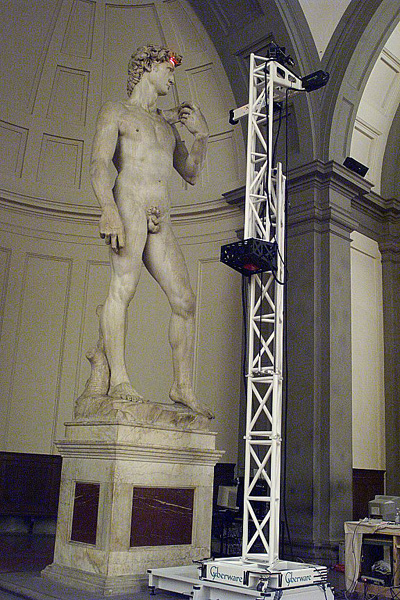
\includegraphics[height=200px]{../images/david_scan.jpg}
\caption{An example of a laser scanner setup used by the Digital Michelangelo Project~\cite{Levoy}.}
\end{figure}

However, laser scanners do have several drawbacks. The equipment is extremely expensive, bulky, and fragile. The Michelangelo Project had to transport over 4 tons of equipment to Italy in order to produce their scans. Additionally, laser scans involve immense setup and can take many hours. The model of David took over a thousand man-hours to scan and even more than that in post processing~\cite{Levoy}.

\subsection{Multi-View Stereo}
Multi-view stereo uses a collection of 2D images to reconstruct a 3D object model. By viewing a single object from hundreds of different camera positions, it is possible to generate a 3D model. Although this technique originally required precisely known camera coordinates, recent algorithms can produce a 3D model from an unordered collection of images with unknown camera positions, assuming that there is sufficient coverage. Existing software packages such as Bundler and Agisoft Photoscan can produce high-quality 3D reconstructions using these unordered image collections~\cite{bundler, Agisoft}.

The ability to use a collection of images without precise camera position information means that these 3D objects can be modeled substantially faster than with a laser scanner. With a smaller object, it is a relatively simple process to take pictures of the object from many different angles. However, for a larger object, such as a statue or building, the task of gathering imagery becomes substantially more difficult.

\begin{figure}
\centering
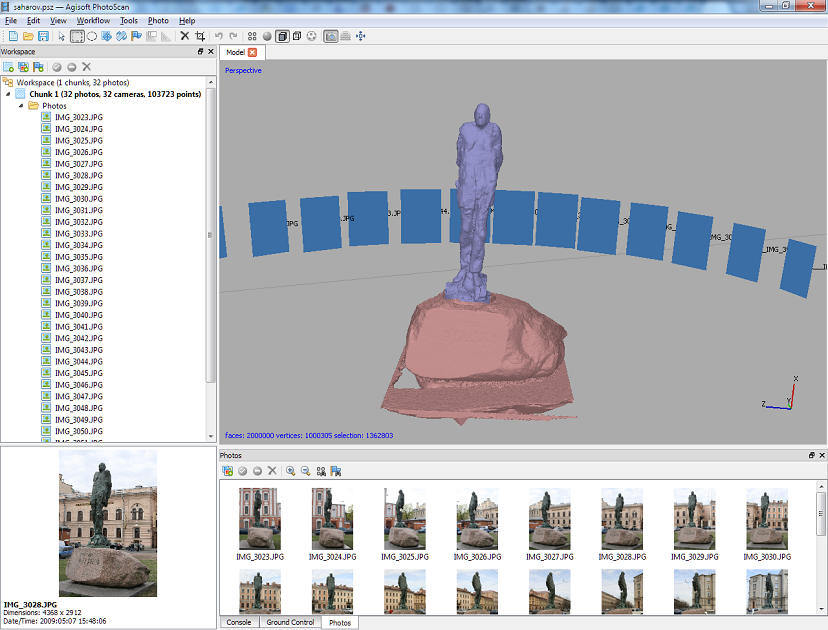
\includegraphics[height=200px]{../images/photoscan.png}
\caption{A 3D model of a statue generated by Agisoft Photoscan. Notice the derived camera planes encompassing the statue~\cite{Agisoft}.}
\end{figure}

\subsection{Microsoft Kinect}

Several groups have researched using the Microsoft Kinect for model acquisition. As the Kinect produces an RGB image with depth information, either the Kinect or the model most be moved in order to produce a complete scan. While this has been found to be useful in scanning small to medium size objects, such as people, the Kinect has several limitations. First of all, the depth range is rather short, on the order of a few meters. Additionally, because the depth is partially determined using an infrared pattern, the Kinect does not work in locations with a large amount of background infrared light, such as outdoors.


\section{Problem Definition}
The goal of this system to capture imagery of large 3D objects for use in multi-view stereo software. This system has several requirements:

\begin{enumerate}
\item
\textbf{Low Cost}

The system should be substantially cheaper than laser scanning.

\item
\textbf{Easy to Use}

This system should be able to be deployed by users with minimal training and setup. Additionally, the hardware should be off-the-shelf and easily accessible.

\item
\textbf{Complete Coverage}

The system must be able to capture images from a wide variety of positions, completely covering every part of the target object.

\item
\textbf{High Quality Imagery}

The system must produce sufficiently high resolution, non-blurry images for use in multi-view stereo software.

\end{enumerate}

\section{Proposed Solution}

We propose using low-cost autonomous quadcopters to gather the imagery needed for use in multi-view stereo software. By flying a quadcopter with a mounted camera around the target object, imagery can quickly be gathered from a wide variety of positions around the object. Using quadcopters has many advantages.

\begin{figure}
\centering
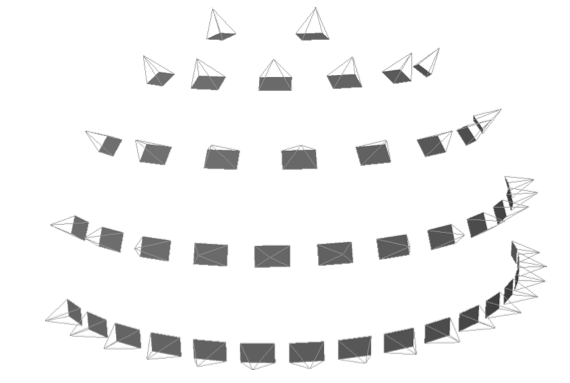
\includegraphics[width=200px]{../images/camera_network.png}
\caption{An example of camera positions for use in multi-view stereo. Such viewpoints could be attained by using quadcopters~\cite{Irschara}.}
\end{figure}

\begin{enumerate}
\item
Quadcopters can capture images from positions unreachable by ground-based cameras.

\item
By methodically flying around the target object at different altitudes, complete coverage of the target object can be achieved.

\item
The imagery can be captured very quickly, on the order of a few minutes.

\item
Quadcopters are small, portable, and easily deployable.


\end{enumerate}

\section{Solution Components}

In order to implement such a solution, there are two main components which must be created. First, a localization algorithm is needed to produce position and orientation estimates of the quadcopter in the global frame. Then, a controller is needed to produce the control inputs for the quadcopter to move in the desired path. This thesis focuses on the design, implementation, and testing of the localization component, while the thesis of Sarah Tang in the Mechanical and Aerospace Engineering Department addresses the controller component of this system.








\chapter{Related Work\label{ch:pastwork}}

This is related work.


\chapter{Conclusion\label{ch:conclusion}}

This thesis proposed a method for 3D model generation using autonomous quadcopters and multi-view stereo. Such a system would be portable, cheap, and easily deployable in a range of applications such as archeology and video game development. 
Specifically, this thesis presented a localization method for low-cost quadcopters using a particle filter with augmented reality tags. This system was shown to perform substantially better than using local sensor measurements alone.

\section{Future Work}

The next step in creating this system for model generation would be to fully integrate this localization algorithm with a controller and path planner. While much effort was put into integrating this work and the controller produced by Sarah Tang, various hardware issues prevented fully autonomous flight from being achieved.

Once basic waypoint tracking is implemented, the system could autonomously generate the path it flies around the object so as too improve coverage and fly around irregularly shaped objects. Eventually, such a system should be packaged in a way such that it can easily be used with the AR.Drone with very little setup, bringing the ability to quickly develop 3D models of large objects to researchers across many fields.
\appendix % all chapters following will be labeled as appendices
\chapter{Implementation\label{ch:implementation}}

% \lstinputlisting{"/Users/ekelley/Google Drive/Projects/QuadcopterMapping/quadcopterCode/src/drone_controller.py"}
% \lstinputlisting{"/Users/ekelley/Google Drive/Projects/QuadcopterMapping/quadcopterCode/src/localize.py"}
% \lstinputlisting{"/Users/ekelley/Google Drive/Projects/QuadcopterMapping/quadcopterCode/src/particlefilter.py"}

\include{ch-appendicies/printing}


% Make the bibliography single spaced
\singlespacing
\bibliographystyle{plain}

% add the Bibliography to the Table of Contents
\cleardoublepage
\ifdefined\phantomsection
  \phantomsection  % makes hyperref recognize this section properly for pdf link
\else
\fi
\addcontentsline{toc}{chapter}{Bibliography}

% include your .bib file
\bibliography{thesis}

\end{document}

